% !TEX root = Krylov_QMC.tex
\section{Computational Results}
\label{sec:results}
In this section we consider an example from
\cite{cesinh}. The formulation of the transport
problem is taken from \cite{ctk:jeff1}. The equation for the angular
flux \(\psi\) is

\begeq
\label{eq:transportgs}
\mu \frac{\partial \psi}{\partial x} (x,\mu) + \Sigma_t(x) \psi(x,\mu) =
\frac{1}{2} \left[ \Sigma_s(x) \int_{-1}^1 \psi(x, \mu') \dmup + q(x) \right]
 \mbox{ for } 0 \le x \le \tau
\endeq

The boundary conditions are

\[
\psi(0, \mu) = \psi_l(\mu), \mu > 0; \psi(\tau, \mu) = \psi_r(\mu),
\mu < 0.
\]

\subsection{Multigroup Equations}
In general geometry the multigroup equations are 
\begin{equation}\label{eq:MG}
\mu  \frac{\partial \psi_g}{\partial x} (x,\mu) + \Sigma_{t,g}(x) \psi_g(x,\mu) =
\frac{1}{2} \sum_{g'=1}^G \Sigma_{s,g'\rightarrow g}(x) \int_{-1}^1 \psi_{g'}(x, \mu') \dmup + \frac{q_g(x)}{2} \quad g=1,\dots,G.
\end{equation}The boundary conditions are
\[
\psi_g(0, \mu) = \psi_{l,g}(\mu), \mu > 0; \psi_g(\tau, \mu) = \psi_{r,g}(\mu),
\mu < 0.
\]
In matrix form, these equations are
\begin{equation}\label{eq:MGmat}
\mu  \frac{\partial \vec{\psi}}{\partial x} (x,\mu) + \underline{\Sigma}_{t}(x) \vec{\psi}(x,\mu) =
\frac{1}{2}  \underline{\Sigma}_{s}(x) \int_{-1}^1 \vec{\psi}(x, \mu') \dmup + \frac{\vec{q}(x)}{2},
\end{equation}
where
\begin{equation}\label{eq:vecs}
\vec{\psi} = (\psi_1, \psi_2, \dots, \psi_G)^\mathrm{T}, \qquad \vec{q} = (q_1, q_2, \dots, q_G)^\mathrm{T}, 
\end{equation}
\begin{equation}\label{eq:MatricesT}
 \underline{\Sigma}_{t}(x)  = \begin{pmatrix} \Sigma_{t,1}(x) & 0 & \dots\\
 0 & \Sigma_{t,2}(x) & 0 \dots \\
 \vdots & & \ddots\\ 
 0 & \dots & 0 & \Sigma_{t,G}(x) 
 \end{pmatrix}, 
\end{equation}
and
\begin{equation}\label{eq:MatricesS}
 \underline{\Sigma}_{s}(x)  = \begin{pmatrix} \Sigma_{s,1\rightarrow 1}(x) & \Sigma_{s,2\rightarrow 1}(x)  & \dots & \Sigma_{s,G\rightarrow 1}(x) \\
 \Sigma_{s,2\rightarrow 1}(x) & \Sigma_{s,2\rightarrow 1}(x)  & \dots & \Sigma_{s,G\rightarrow 2}(x) \\
 \vdots & \vdots & & \vdots\\
 \Sigma_{s,G\rightarrow 1}(x) & \Sigma_{s,G\rightarrow 1}(x)  & \dots & \Sigma_{s,G\rightarrow G}(x) \\
 \end{pmatrix},.
\end{equation}

\subsection{Source Iteration and Linear Solvers}
\label{subsec:source}

Source iteration is Picard iteration for the fixed point problem
\[
\phi = \cals(\phi, q, \psi_l, \psi_r)
\]
To use other solvers we must convert to a linear system via
\[
\calk(\phi) = \cals(\phi, 0, 0, 0) \mbox{ and }
f = \cals(0, q, \psi_l, \psi_r)
\]
to get
\[
A \phi \equiv (I - \calk) \phi = f,
\]
which we can send to a linear solver.

In the computations we use the problem from \cite{cesinh}
\[
\tau=5, \Sigma_s(x) =\omega_0 e^{-x/s},  \Sigma_t(x) = 1, q(x) = 0, \psi_l(\mu) = 1, \psi_r(\mu) = 0,
\]
and consider two cases $s=1$ and $s=\infty$ 

\clearpage

\subsection{QMC and Krylov Linear Solvers}
\label{subsec:krylov}


The linear and nonlinear solvers come from the Julia package
\href{https://github.com/ctkelley/SIAMFANLEquations.jl}{SIAMFANLEQ.jl}
\cite{ctk:siamfanl}. The documentation for these codes is in the
\href{https://github.com/ctkelley/NotebookSIAMFANL}{Juila notebooks}
\cite{ctk:notebooknl} and the book \cite{ctk:fajulia}
that accompany the package. 

For each example,
we use two Krylov methods \cite{ctk:roots}, GMRES \cite{gmres} and
Bi-CGSTAB \cite{bicgstab}.  

\subsubsection{Garcia-Siewert}

We solve the QMC linear problem with N=2048 and Nx= 100. 
Figures~\ref{fig:easy} and 
\ref{fig:hard} show that
the Krylov iterations take fewer than half of the number
of transport sweeps that Picard iteration required.

\vspace*{.25in}

\begin{figure}[h]
\centerline{
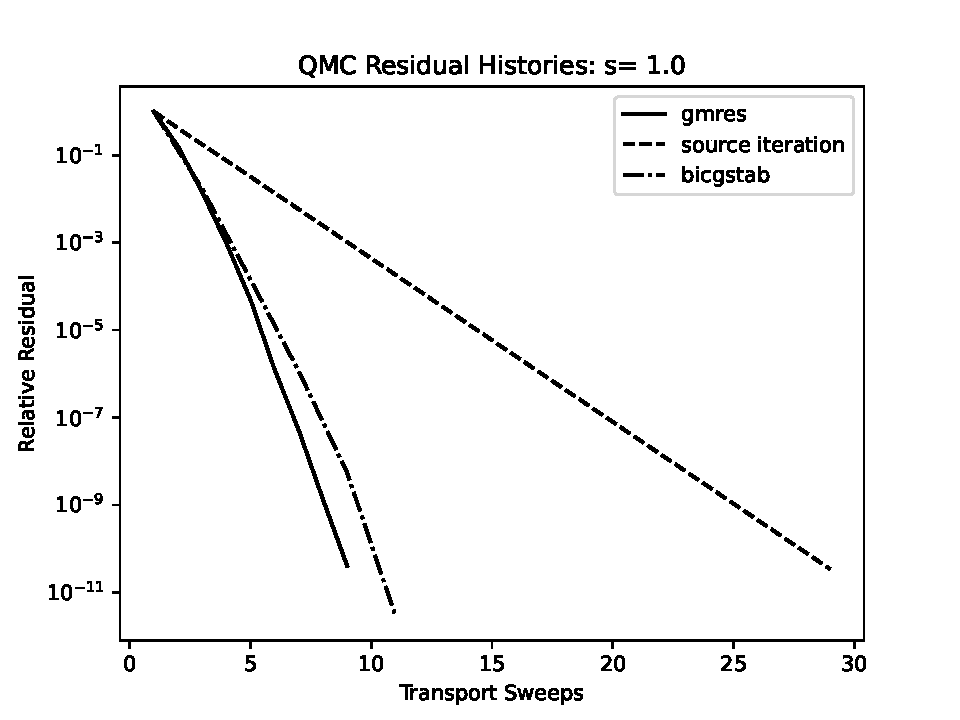
\includegraphics[width=3.5in]{FIGURES/seqone.pdf}
}
\caption{\label{fig:easy} $s=1$}
\end{figure}

\begin{figure}[h]
\centerline{
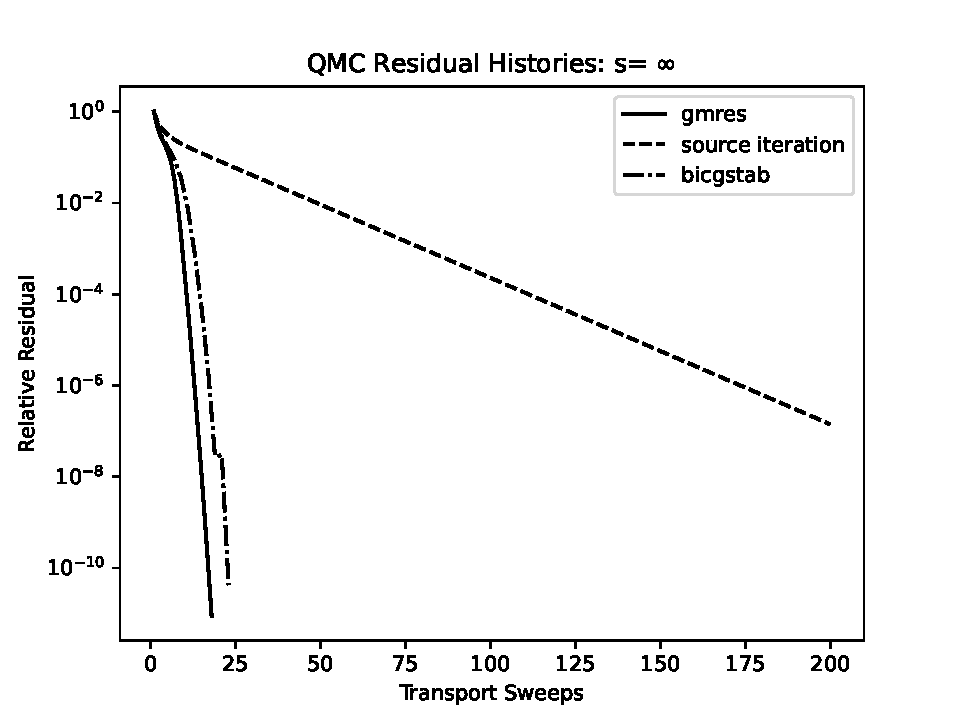
\includegraphics[width=3.5in]{FIGURES/seqinf.pdf}
}
\caption{\label{fig:hard} $s=\infty$}
\end{figure}

\clearpage

\subsection{Validation and calibration study}
\label{validation-and-calibration-study}

We conclude this section with a validation study. We compare the
QMC results with the results from \cite{cesinh}. The results
in \cite{cesinh} are exit distributions and are accurate to 
six figures. We have duplicated those results with an $Sn$ computation
on a fine angular and spatial mesh.

{\bf Sam, Ryan, should we use more or different values of $N$ and $Nx$?}

For $N = 2048$ and $Nx=100$ we obtain the cell-average fluxes from
the QMC approximation. We then use a single Sn transport sweep to recover
the exit distributions from the QMC cell-average fluxes. We report
the results and the corresponding results from \cite{cesinh} in 
Tables~\ref{tab:cesone} and \ref{tab:cesinf}.

The exit distributions, as is clear from Table~\ref{tab:cesone}
can vary by five orders of magnitude. Even so, the results from QMC
agree with the benchmarks to roughly two figures.

\begin{table}[h]
\centering
\caption{Exit Distributions: $s = 1$}
\label{tab:cesone}
\centerline{
\begin{tabular}{lllll}
 & \multicolumn{2}{c}{Garcia/Siewert}
 & \multicolumn{2}{c}{QMC}\\
\hline
$\mu$ &$\psi(0, -\mu)$ &$\psi(\tau, \mu)$ &$\psi(0, -\mu)$ &$\psi(\tau, \mu)$ \\
\hline
 0.05 &    5.89664e-01 &    6.07488e-06 &    6.07035e-01 &    5.91908e-06   \\ 
 0.10 &    5.31120e-01 &    6.92516e-06 &    5.47466e-01 &    6.74075e-06   \\ 
 0.20 &    4.43280e-01 &    9.64232e-06 &    4.57064e-01 &    9.35453e-06   \\ 
 0.30 &    3.80306e-01 &    1.62339e-05 &    3.92223e-01 &    1.56108e-05   \\ 
 0.40 &    3.32964e-01 &    4.38580e-05 &    3.43481e-01 &    4.13721e-05   \\ 
 0.50 &    2.96090e-01 &    1.69372e-04 &    3.05510e-01 &    1.58622e-04   \\ 
 0.60 &    2.66563e-01 &    5.73465e-04 &    2.75098e-01 &    5.39514e-04   \\ 
 0.70 &    2.42390e-01 &    1.51282e-03 &    2.50192e-01 &    1.43257e-03   \\ 
 0.80 &    2.22235e-01 &    3.24369e-03 &    2.29422e-01 &    3.08975e-03   \\ 
 0.90 &    2.05174e-01 &    5.96036e-03 &    2.11837e-01 &    5.70555e-03   \\ 
 1.00 &    1.90546e-01 &    9.77123e-03 &    1.96756e-01 &    9.39189e-03   \\ 
\hline
\end{tabular}
}
\end{table}


\begin{table}[h]
\centering
\caption{Exit Distributions: $s = \infty$}
\label{tab:cesinf}
\begin{tabular}{lllll}
 & \multicolumn{2}{c}{Garcia/Siewert}
 & \multicolumn{2}{c}{QMC}\\
\hline
$\mu$ &$\psi(0, -\mu)$ &$\psi(\tau, \mu)$ &$\psi(0, -\mu)$ &$\psi(\tau, \mu)$ \\
\hline
0.05 &    8.97798e-01 &    1.02202e-01 &    9.06050e-01 &    1.03680e-01   \\ 
 0.10 &    8.87836e-01 &    1.12164e-01 &    8.95849e-01 &    1.13695e-01   \\ 
 0.20 &    8.69581e-01 &    1.30419e-01 &    8.76487e-01 &    1.31907e-01   \\ 
 0.30 &    8.52299e-01 &    1.47701e-01 &    8.58937e-01 &    1.49245e-01   \\ 
 0.40 &    8.35503e-01 &    1.64497e-01 &    8.42195e-01 &    1.66128e-01   \\ 
 0.50 &    8.18996e-01 &    1.81004e-01 &    8.25870e-01 &    1.82734e-01   \\ 
 0.60 &    8.02676e-01 &    1.97324e-01 &    8.09780e-01 &    1.99151e-01   \\ 
 0.70 &    7.86493e-01 &    2.13507e-01 &    7.93834e-01 &    2.15421e-01   \\ 
 0.80 &    7.70429e-01 &    2.29571e-01 &    7.77997e-01 &    2.31558e-01   \\ 
 0.90 &    7.54496e-01 &    2.45504e-01 &    7.62269e-01 &    2.47547e-01   \\ 
 1.00 &    7.38721e-01 &    2.61279e-01 &    7.46673e-01 &    2.63362e-01   \\ 
\hline
\end{tabular}
\end{table}

In Tables \ref{tab:bigtab1} and \ref{tab:bigtabinf} we look at the
relative errors in the QMC exit distributions as compared to a highly
accurate SN result. We compensate for the widely varying scales by tabulating,
for each value of $N$ and $Nx$
\[
R = \max(R^0, R^\tau)
\]
where
\[
R^0 = \max_\mu
\frac{ | \psi^{SN}(0,-\mu) - \psi^{QMC}(0,-\mu) | }{\psi^{SN}(0,-\mu) }
\]
and
\[
R^\tau = \max_\mu
\frac{ | \psi^{SN}(\tau,\mu) - \psi^{QMC}(\tau,\mu) | }{\psi^{SN}(\tau,\mu) }.
\]

{\bf Ryan, for large Nx I see convergence as N increases. Is it clearly
$1/N$? Am I missing something? Am I tabulating the wrong thing?}

\begin{table}[h]
\centering
\caption{Exit Distributions Errors: $s = 1.0$}
\label{tab:bigtab1}
\begin{tabular}{l|lllll} 
\hline
 Nx \textbackslash N &     1024 &     2048 &     4096 &     8192 &    16384 \\ 
\hline 
50 & 1.31716e-01& 1.34260e-01& 1.35123e-01& 1.35328e-01& 1.35242e-01   \\ 
100 & 6.09631e-02& 6.35764e-02& 6.46191e-02& 6.48898e-02& 6.48536e-02   \\ 
200 & 3.77223e-02& 3.12496e-02& 3.12005e-02& 3.17337e-02& 3.16710e-02   \\ 
400 & 2.63214e-02& 1.45106e-02& 1.52355e-02& 1.56636e-02& 1.56854e-02   \\ 
800 & 2.39486e-02& 9.94925e-03& 7.24627e-03& 8.86212e-03& 7.84063e-03   \\ 
1600 & 4.16277e-02& 9.95048e-03& 5.11618e-03& 8.02709e-03& 4.44021e-03   \\ 
3200 & 4.60905e-02& 1.07345e-02& 4.45922e-03& 7.49522e-03& 3.76179e-03   \\ 
\hline 
\end{tabular} 
\end{table}

\begin{table}[h]
\centering
\caption{Exit Distributions Errors: $s = \infty$}
\label{tab:bigtabinf}
\begin{tabular}{l|lllll} 
\hline
 Nx \textbackslash N &     1024 &     2048 &     4096 &     8192 &    16384 \\ 
\hline 
50 & 1.31716e-01& 1.34260e-01& 1.35123e-01& 1.35328e-01& 1.35242e-01   \\ 
100 & 6.09631e-02& 6.35764e-02& 6.46191e-02& 6.48898e-02& 6.48536e-02   \\ 
200 & 3.77223e-02& 3.12496e-02& 3.12005e-02& 3.17337e-02& 3.16710e-02   \\ 
400 & 2.63214e-02& 1.45106e-02& 1.52355e-02& 1.56636e-02& 1.56854e-02   \\ 
800 & 2.39486e-02& 9.94925e-03& 7.24627e-03& 8.86212e-03& 7.84063e-03   \\ 
1600 & 4.16277e-02& 9.95048e-03& 5.11618e-03& 8.02709e-03& 4.44021e-03   \\ 
3200 & 4.60905e-02& 1.07345e-02& 4.45922e-03& 7.49522e-03& 3.76179e-03   \\ 
\hline 
\end{tabular} 
\end{table}

\subsubsection{Multigroup Problems}

These are preliminary results with $N_x = 40$ and $N=2^{10}$. We may
want to make these larger and/or make tables like 
Table~\ref{tab:bigtab1} and Table~\ref{tab:bigtab1}. 

\begin{figure}[h]
\centerline{
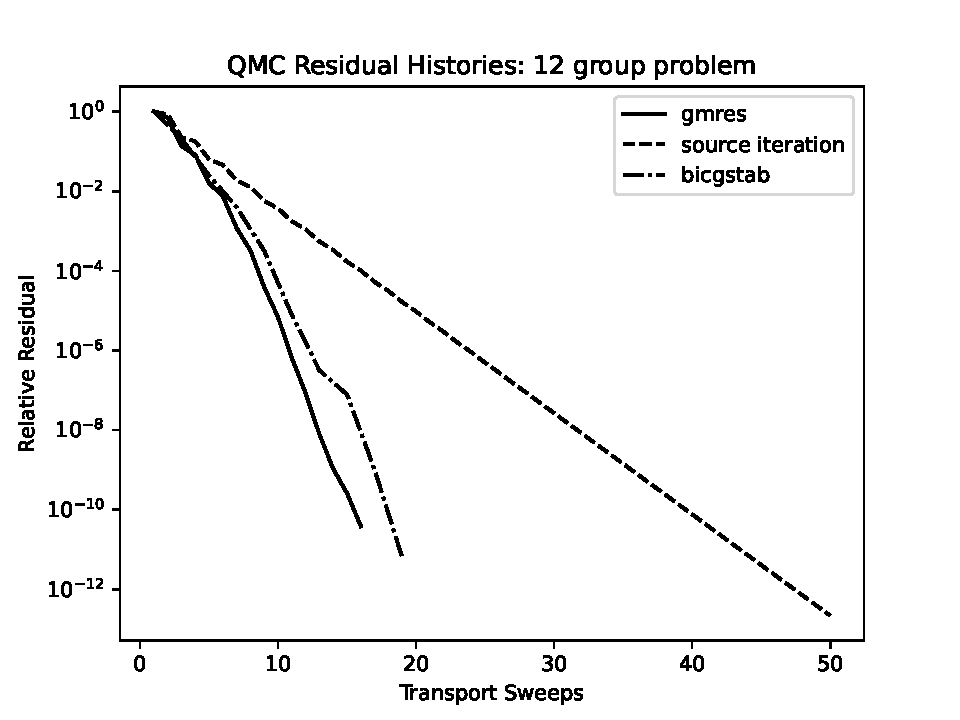
\includegraphics[width=3.5in]{FIGURES/12Group.pdf}
}
\caption{\label{fig:12group}}
\end{figure}

\begin{figure}[h]
\centerline{
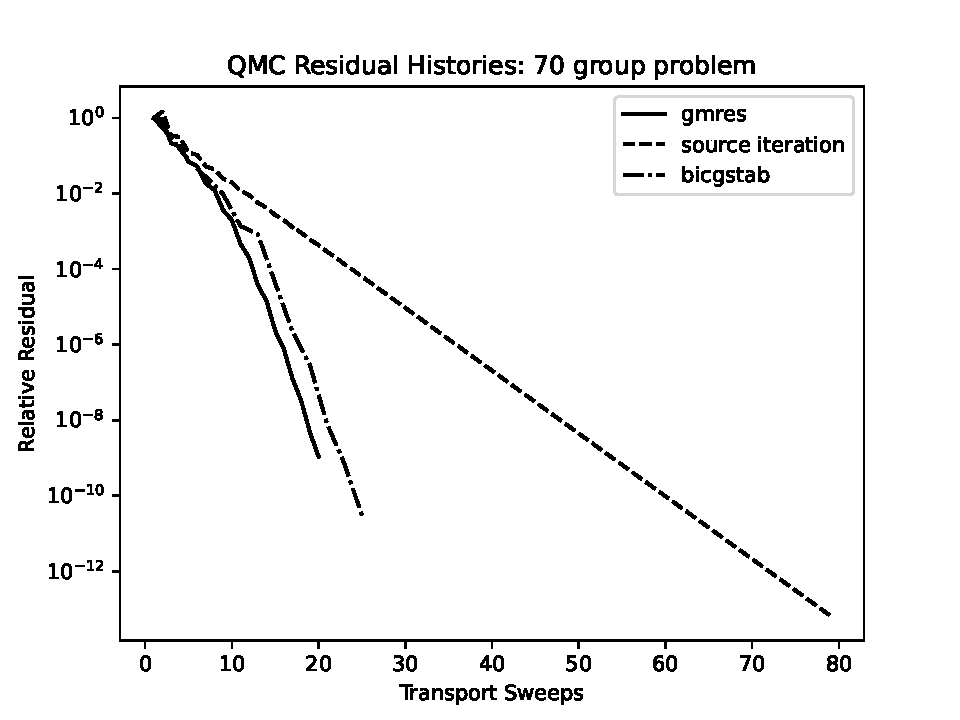
\includegraphics[width=3.5in]{FIGURES/70Group.pdf}
}
\caption{\label{fig:70group}}
\end{figure}

\begin{figure}[h]
\centerline{
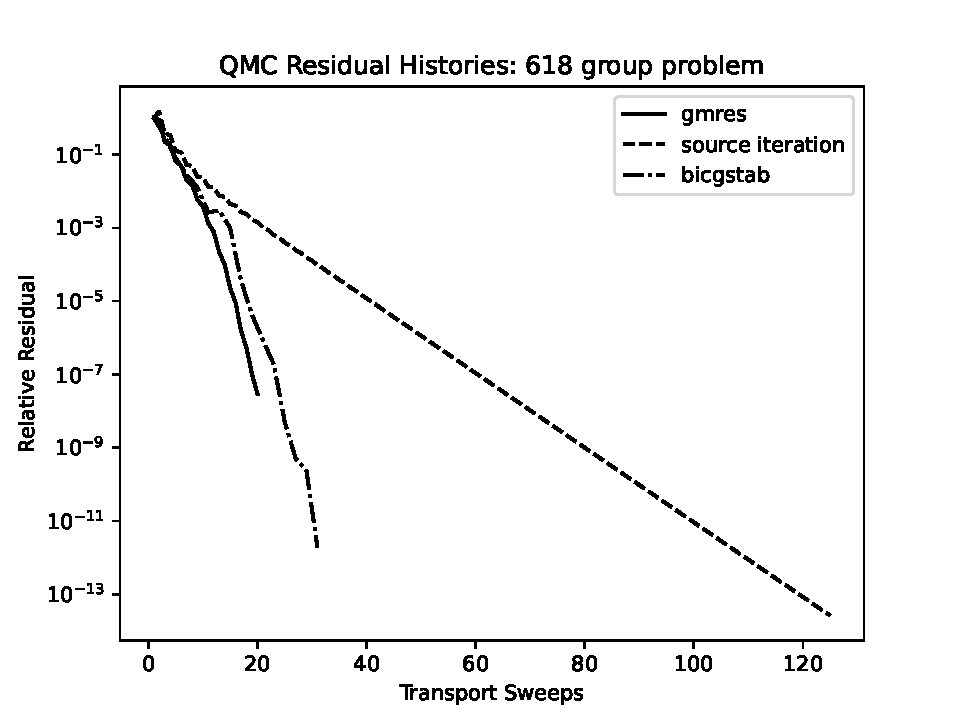
\includegraphics[width=3.5in]{FIGURES/618Group.pdf}
}
\caption{\label{fig:618group}}
\end{figure}


